\chapter{Introdução}
\label{chap:introducao}

O presente capítulo visa fornecer uma visão geral que enquadra e organiza os diferentes aspetos que serão aprofundados nas secções subsequentes.

No seu conteúdo, apresenta-se o enquadramento e a relevância do projeto desenvolvido no âmbito da unidade curricular de Projeto Estágio (PESTI). Este trabalho integrou-se no programa internacional Blended4Future, uma iniciativa que reúne estudantes de diversas instituições europeias com o propósito de promover o desenvolvimento de competências técnicas e colaborativas através da realização de projetos aplicados a necessidades reais de empresas parceiras.

Serão descritos o contexto em que o projeto foi concebido, o problema central identificado e os objetivos definidos para a sua resolução. Além disso, explicita-se a organização da equipa de trabalho e a metodologia adotada para guiar o processo de desenvolvimento.

Por último, apresentam-se as principais tecnologias selecionadas para a implementação da solução e faz-se referência aos desafios mais significativos enfrentados ao longo da execução do projeto.



\section{Enquadramento}
\label{sec:introducao_enquadramento}

Este relatório foi desenvolvido com base num projeto enquadrado no âmbito da unidade curricular de Projeto Estágio (PESTI) da Licenciatura em Engenharia Informática (LEI) do Instituto Superior de Engenharia do Porto (ISEP).

Este projeto ocorreu no enquadramento do Projeto BlendED (também referido como Blended4Future ou BlendedMobility\footnote{https://blendedmobility.com}). Este curso dá a estudantes a oportunidade de desenvolverem as suas \textit{soft} e \textit{hard skills} num projeto com alunos de diferentes culturas e países trabalhando num ambiente para empresas reais.

\subsection{Apresentação da organização}

BlendedMobility é uma iniciativa educativa internacional que promove o desenvolvimento de projetos colaborativos no contexto do ensino híbrido. Esta visa combinar experiências de aprendizagem presencial e \textit{online}, proporcionando aos estudantes uma formação mais flexível, personalizada e orientada para a prática.

O programa reúne alunos de diferentes universidades europeias que, ao longo de quatro meses, trabalham em conjunto no desenvolvimento de projetos reais para empresas parceiras. A metodologia adotada assenta em práticas ativas e colaborativas, potenciando competências essenciais como trabalho em equipa, comunicação intercultural e resolução de problemas num ambiente profissional simulado.

O percurso iniciou-se com uma semana presencial no Instituto Universitário da Maia (ISMAI), onde as equipas se conheceram, receberam o enquadramento do projeto e planearam as etapas de trabalho. O desenvolvimento dos projetos decorreu num regime híbrido, combinando sessões \textit{online} e trabalho autónomo. Ao final do ciclo, todas as equipas reuniram-se presencialmente na Universidade de Trier, na Alemanha, para apresentar os resultados dos seus projetos a um painel de avaliadores e representantes das empresas envolvidas.


\section{Descrição do Problema}
\label{sec:introducao_descproblema}

O Website do curso Blended4Future estava muito aquém do espectado, muitos elementos seguiam um design inconsistente e antiquado, ou não estavam completamente funcionais. 

A organização desejava uma plataforma onde se pudesse automaticamente adicionar projetos, alunos, universidades e empresas numa só plataforma. Por tal foi colocada uma proposta de desenvolvimento de uma nova aplicação \textit{web} que substituiria esta anterior. 

Nesta aplicação, estudantes professores e representantes de empresas poderiam ver os projetos em que estavam envolvidos e fazer posts sobre os seus respetivos projetos.

Foi ainda requisitada a criação de uma ferramenta para visualizar todas a edições do Blended4Future e todos os projetos neste envolvido.

\section{Objetivos}

A aplicação web a desenvolver deverá incluir um sistema de autenticação com diferenciação entre perfis de utilizador, nomeadamente administradores e utilizadores comuns, assegurando uma gestão adequada de permissões. 

Adicionalmente, deverá permitir a criação de novos projetos e a associação de diferentes intervenientes a cada um, consoante o seu papel. Além disso, deverá ser implementada uma biblioteca de projetos, acessível a qualquer utilizador da plataforma, onde estarão disponíveis todos os projetos desenvolvidos no âmbito do curso, promovendo a sua consulta e divulgação.

A interface da aplicação deverá seguir as diretrizes de design definidas previamente por um membro da equipa dedicado ao design visual da aplicação.


\section{Abordagem}

\subsection{A equipa}

A equipa foi composta por um grupo de estudantes provenientes de várias universidades europeias, com a seguinte constituição:

\begin{itemize}
    \item 5 Engenheiros de \textit{software}
    \item 1 \textit{Designer}
    \item 1 \textit{Marketer}
\end{itemize}

A equipa de IT, constituída por cinco engenheiros de \textit{software}, foi organizada em duas subequipas: 
\begin{itemize}
    \item 3 estudantes dedicados ao desenvolvimento de \textit{Backend}
    \item 2 estudantes dedicados ao desenvolvimento de \textit{Frontend}, incluindo o autor deste relatório, que integrou esta subequipa para participar no desenvolvimento da interface de utilizador.
\end{itemize}

Esta divisão teve como objetivo garantir um maior avanço na lógica de negócio durante a fase inicial do projeto. 
Numa etapa posterior, quando a lógica estivesse próxima da sua conclusão, alguns dos estudantes poderiam transitar para a subequipa de \textit{Frontend}, focando-se então na criação da interface de utilizador.

É importante salientar que, no âmbito do projeto Blended4Future, cada estudante participa com um número distinto de créditos (ECTS), definidos em função de uma unidade curricular do seu respetivo curso, afetando assim a respetiva carga horária no trabalho. Assim, tornou-se necessário organizar a distribuição das tarefas de forma proporcional, garantindo que a carga de trabalho atribuída a cada elemento refletisse adequadamente o valor dos créditos em que estava inscrito.

\subsection{Metodologia de trabalho}

Para uma melhor organização do trabalho, foi adotada a metodologia Scrum, com sprints de duas semanas de duração. Além disso, foi estabelecida, por consenso do grupo, a realização de reuniões semanais para atualizar o progresso das tarefas e promover um ambiente de trabalho mais colaborativo e comunicativo. Estas reuniões não possuíam uma data definida tendo em conta os fusos horários de cada um dos membros.

\subsubsection{Divisão de sprints}

A Tabela \ref{tab:organizacao_sprints} demonstra a divisão de sprints feita. Foi ainda definido objetivos para os primeiros quatro sprints.

\paragraph*{Objetivos Sprint 1–2}
\begin{itemize}[nosep,leftmargin=*]
  \item Documentação geral do projeto
  \item Configuração dos repositórios de Backend/Frontend
    \begin{itemize}[nosep,leftmargin=*]
      \item Pipelines de CI/CD
    \end{itemize}
  \item Configuração de DevOps/Azure
  \item Análise SWOT do negócio
\end{itemize}

\paragraph*{Objetivos Sprint 3–4}
\begin{itemize}[nosep,leftmargin=*]
  \item Finalização da documentação geral
  \item Início do desenvolvimento
\end{itemize}
%tab:organizacao_sprints
\begin{table}[h!tbp]
    \centering
    \caption{Organização de sprints definida pela equipa}
    \begin{tabular}{llll}
        Sprint & Semanas & Data de início & Data de fim \\\midrule
        1      & 1-2     & 24/02          & 02/03       \\\midrule
        2      & 3-4     & 10/03          & 23/03       \\\midrule
        3      & 5-6     & 24/03          & 06/04       \\\midrule
        4      & 7-8     & 07/04          & 20/04       \\\midrule
        5      & 9-10    & 21/04          & 04/05       \\\midrule
        6      & 11-12   & 05/05          & 18/05       \\\midrule
        7      & 13-14   & 19/05          & 01/06       \\\midrule
        8      & 15-16   & 02/06          & 15/06       \\\bottomrule
    \end{tabular}
    
    \label{tab:organizacao_sprints}
\end{table}


\subsection{Tecnologias Definidas}

Durante a semana de kickoff tornou-se necessário deliberar sobre as tecnologias e ferramentas a adotar para o desenvolvimento do projeto. Ao longo da execução, foram incorporadas soluções adicionais visando otimizar processos e aumentar a eficiência do trabalho realizado.

\subsubsection{Ferramentas de Gestão de projetos}

Primeiramente foi necessário definir uma plataforma central para onde cada elemento do grupo pudesse ver o estado do projeto, incluindo ainda a totalidade do \textit{product backlog}, as suas respetivas tarefas, duração dos sprints e onde se pudesse ter acesso a todos os repositórios necessários ao projeto.

Por aconselhamento dos professores membros do projeto foi escolhido a aplicação da \textit{Azure DevOps}. (Ver Figuras \ref{fig:devops-homepage} e \ref{fig:devops-boards})

Esta ferramenta destaca-se como uma plataforma integrada que oferece um equilíbrio entre funcionalidades avançadas e facilidade de utilização, suportando todo o ciclo de vida do desenvolvimento de software. A sua interface intuitiva, combinada com um elevado grau de personalização dos painéis de trabalho, automações eficazes e relatórios detalhados, facilita a gestão ágil e a integração com o ecossistema Microsoft, bem como com diversas outras ferramentas DevOps. 

\begin{figure}[h!tbp]
    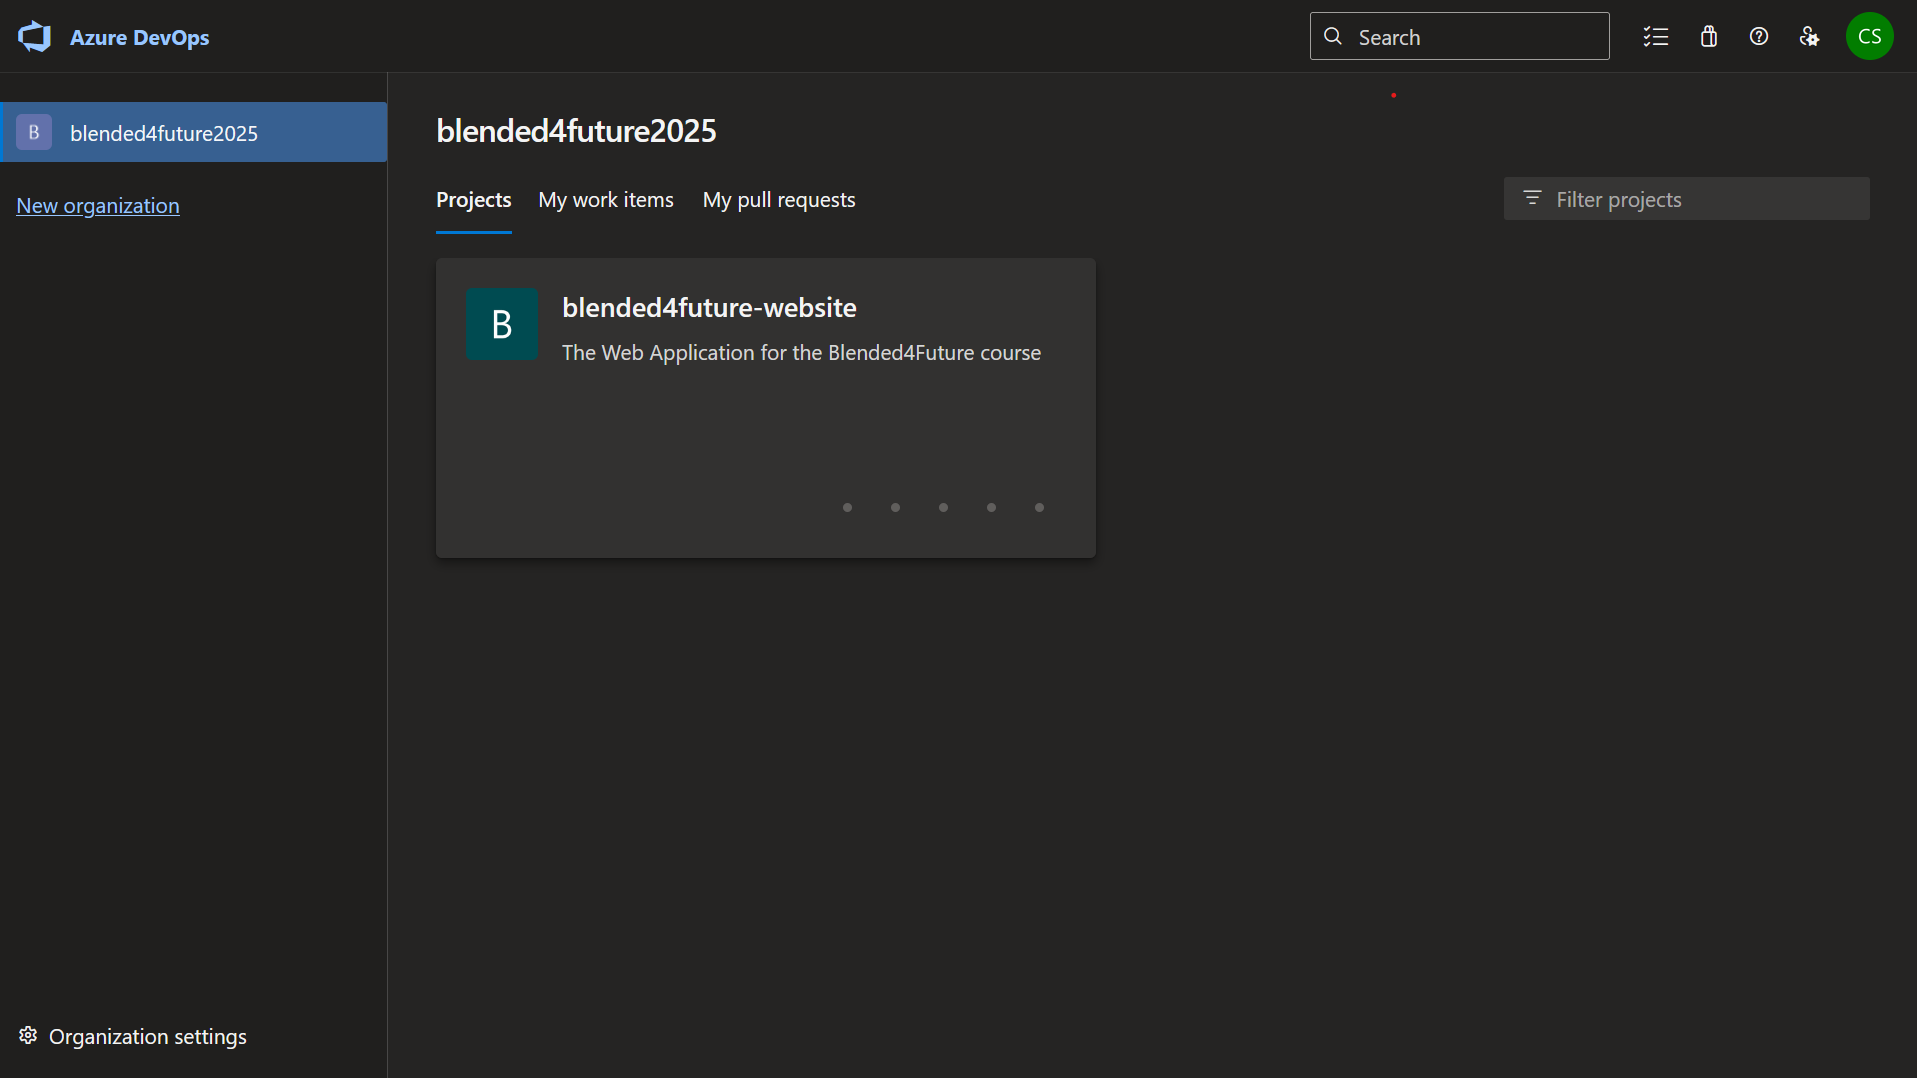
\includegraphics[width=\linewidth]{capitulos/cap1-introducao/imagens/ferramentas/devops-homepage.png}
    \caption{Homepage do projeto}
    \label{fig:devops-homepage}
\end{figure}

\begin{figure}[h!tbp]
    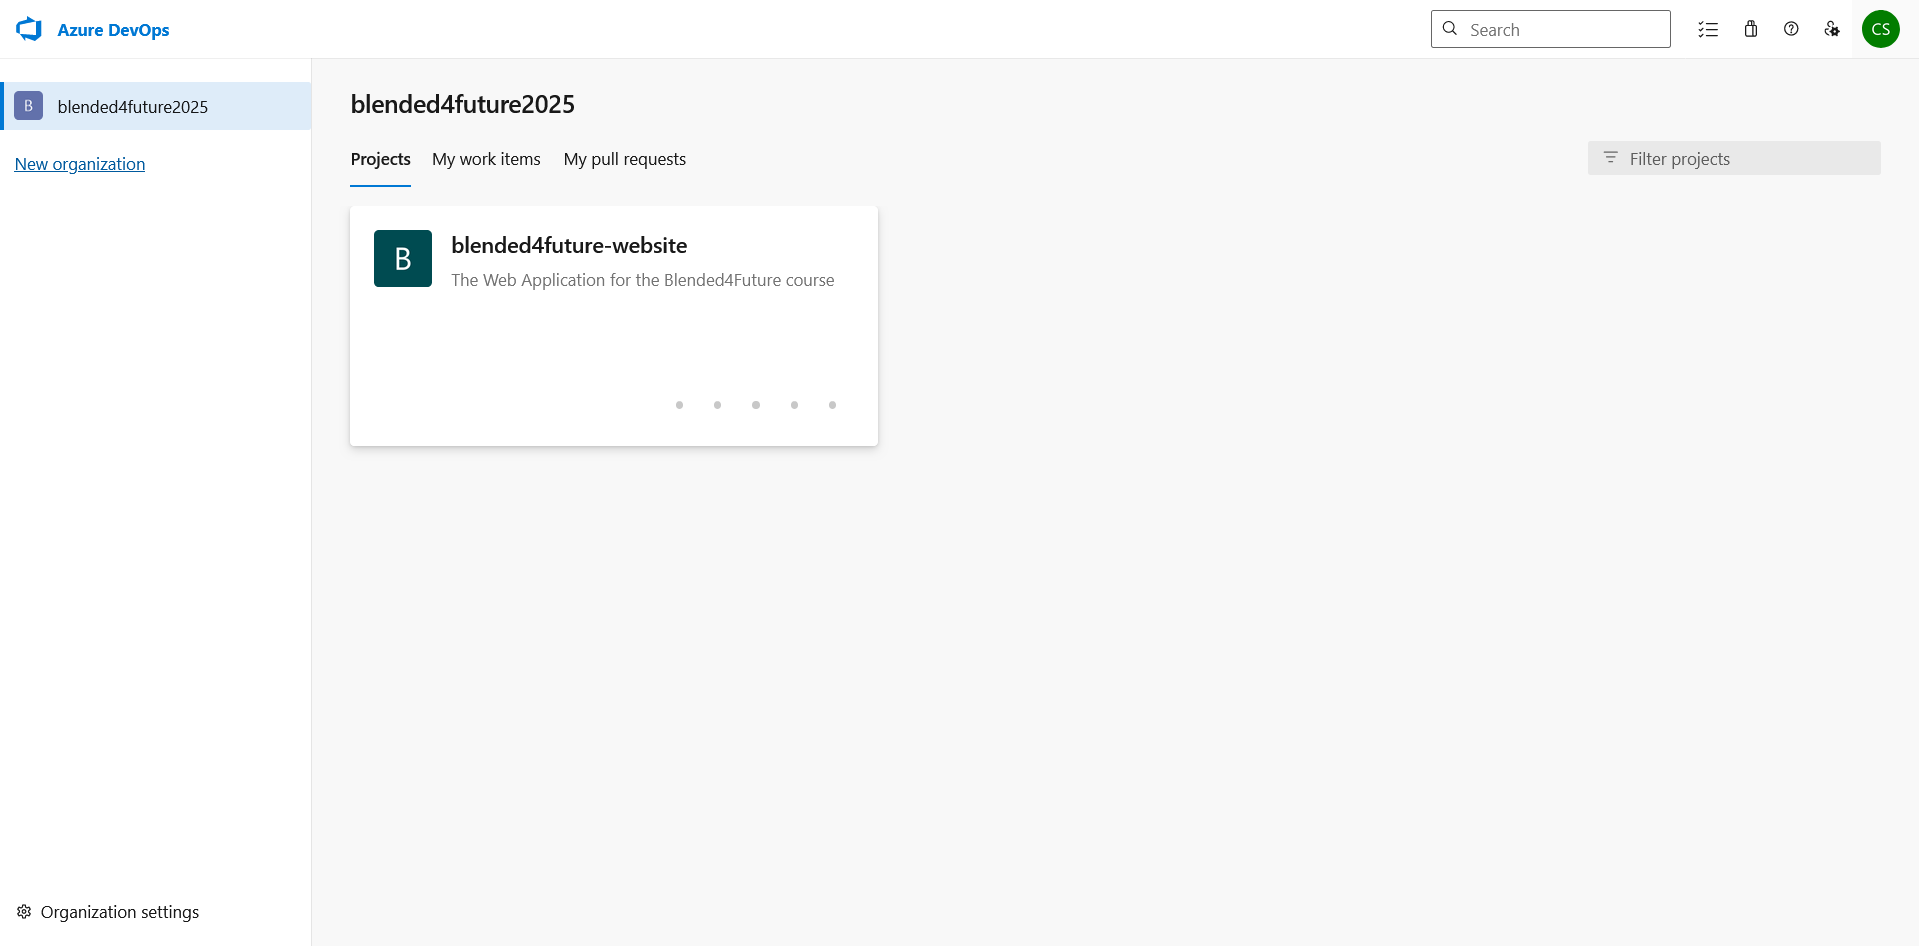
\includegraphics[width=\linewidth]{capitulos/cap1-introducao/imagens/ferramentas/devops-board.png}
    \caption{Exemplificação do uso das \textit{boards} no DevOps}
    \label{fig:devops-boards}
\end{figure}

Outras possíveis e válidas escolhas para este tipo de ferramenta seriam, por exemplo:

\paragraph{Github Projects}

Conhecido pela sua simplicidade e integração direta no ambiente de desenvolvimento, o GitHub Projects permite um acompanhamento natural e ágil das tarefas dentro dos próprios repositórios de código. Esta característica potencia a colaboração entre programadores e torna a ferramenta particularmente útil para projetos de pequena escala ou equipas que privilegiam a rapidez e a facilidade de uso. No entanto, apresenta limitações em termos de funcionalidades de gestão ágil e geração de relatórios detalhados, pelo que pode não ser adequado para projetos com requisitos organizacionais mais rigorosos ou estruturas de equipa complexas.

\paragraph{Jira}

O Jira apresenta-se como uma ferramenta de gestão de projetos altamente robusta, especialmente orientada para equipas que adotam metodologias ágeis, como Scrum e Kanban. Destaca-se pela capacidade de personalização detalhada dos fluxos de trabalho, pela integração aprofundada com ferramentas DevOps e pela produção de relatórios analíticos complexos, que facilitam o acompanhamento rigoroso do progresso em projetos de elevada complexidade. Contudo, a sua curva de aprendizagem é acentuada e a interface pode revelar-se excessivamente densa para utilizadores menos experientes, o que implica um investimento significativo em configuração e formação inicial, podendo limitar a sua eficiência em equipas pequenas ou com recursos reduzidos.


\subsubsection{Tecnologias para desenvolvimento}

Atendendo à heterogeneidade da equipa, composta por indivíduos com diferentes experiências, origens académicas e nacionalidades, tornou-se imperativo definir consensualmente as tecnologias a utilizar no projeto. Para tal, procedeu-se ao levantamento sistemático das ferramentas previamente utilizadas pelos elementos da equipa, tendo-se optado pelas tecnologias mais referidas e consideradas mais adequadas à criação de interfaces de utilizador e à implementação de APIs do tipo REST. 

Importa referir que os restantes elementos da equipa possuíam pouca experiência tanto no desenvolvimento de APIs REST como na construção de interfaces de utilizador. Por essa razão, tornou-se necessária uma etapa inicial de adaptação e aprendizagem, para garantir o domínio das tecnologias que serão posteriormente abordadas.

Houve uma clara preferência quanto ao uso de linguagens com tipagem forte\footnote{Uma linguagem de programação de tipagem forte é aquela em que o sistema de tipos impõe restrições rígidas à forma como valores de tipos diferentes podem ser combinados ou convertidos, evitando conversões implícitas inseguras e reduzindo a ocorrência de erros de tipo em \textit{runtime}.}. Estas permitem o melhor rastreamento de erros e garantem o formato dos objetos no programa. Esta preferência teve como base principal a inexperiência de vários elementos da equipa.

A Tabela \ref{tab:tecnologias-mais-utilizadas} demonstra este levantamento que permitiu à equipa fundamentar a decisão sobre as tecnologias a adoptar:


\begin{table}[h!tbp]
    \centering
    
    \caption{Levantamento das tecnologias que os elementos da equipa já utilizaram}

    \begin{tabular}{ll}
        \toprule
        Tecnologia & Nº de referências \\
        \midrule
        Java & 5 \\
        Python & 4 \\
        CSS & 4 \\
        MySQL & 4 \\
        HTML & 5 \\
        SQL Server & 3 \\
        C & 2 \\
        JavaScript & 5 \\
        TypeScript & 2 \\
        C++ & 2 \\
        Bash Scripting & 1 \\
        R & 1 \\
        ReactTS & 1 \\
        C\# & 1 \\
        .NET (ASP) & 1 \\
        Entity Framework & 1 \\
        H2 & 1 \\
        MongoDB & 1 \\
        PHP & 1 \\
        \bottomrule
    \end{tabular}


    \label{tab:tecnologias-mais-utilizadas}

\end{table}



\paragraph{Java} Linguagem de programação orientada a objetos amplamente utilizada no desenvolvimento de aplicações empresariais e sistemas robustos. A sua integração com o ecossistema Spring possibilita a criação eficiente de APIs REST, suportando a escalabilidade e manutenção do software. A sua tipagem forte permite que erros sejam mais fáceis de evitar, principalmente para desenvolvedores com pouca experiência.  

\subparagraph{Spring} Framework para a plataforma Java caracterizada pela sua modularidade e flexibilidade, que simplifica o desenvolvimento de aplicações empresariais. Entre as suas principais vantagens técnicas destacam-se a Inversão de Controlo e a Injeção de Dependência, que promovem baixo acoplamento e facilitam a manutenção e testabilidade do código. Suporta também Programação Orientada a objetos, permitindo isolar funcionalidades transversais como segurança e logging. Entras a suas várias funcionalidades denota-se o Spring Data, que abstrai o acesso a repositórios e bases de dados, facilitando a interação com diversos sistemas de armazenamento por meio de interfaces padronizadas; assim, os repositórios do Spring permitem a execução simplificada de operações CRUD e consultas complexas sem necessidade de escrever código SQL.

\subparagraph{Junit} Framework amplamente utilizada no desenvolvimento Java para a criação de testes unitários, essencial para garantir a qualidade e fiabilidade do código ao permitir a verificação automática e recetível do comportamento de unidades individuais numa aplicação. Este framework proporciona uma estrutura simples e eficiente para escrever, organizar e executar testes, suportando anotações que facilitam a definição de métodos de teste, fases de inicialização e limpeza, bem como a gestão de exceções esperadas.

\paragraph{TypeScript} Linguagem de programação baseada em JavaScript, que integra tipagem estática e recursos avançados, facilitando o desenvolvimento de interfaces de utilizador complexas e a manutenção de grandes bases de código. A sua adoção é relevante na construção de aplicações web modernas e escaláveis.

\subparagraph{React TS} Framework de desenvolvimento frontend baseada em componentes, que alia a flexibilidade do React à segurança oferecida pela tipagem forte do TypeScript. Esta combinação permite construir interfaces de utilizador dinâmicas e com maior robustez, suportando os modernos paradigmas de desenvolvimento web com principal foco na reusabilidade dos referidos componentes.

\subparagraph{TailwindCSS} Framework utilitária que simplifica a estilização ao permitir aplicar classes diretamente nos componentes de React, eliminando a necessidade de escrever CSS tradicional. A sua integração assegura uma personalização rápida e responsiva, facilitada pela configuração flexível e pelo suporte a interfaces modulares e tipadas com TypeScript, promovendo assim maior produtividade e manutenção eficiente do código em projetos modernos de frontend.

\paragraph{MySQL}: Sistema de gestão de bases de dados relacionais (SGBDR) amplamente utilizado, reconhecido pela sua natureza \textit{open source} e pelo desempenho eficiente em operações de leitura e escrita, particularmente em aplicações web. Entre as suas vantagens técnicas destaca-se a facilidade de uso, a escalabilidade para lidar com grandes volumes de dados e o suporte a transações ACID. Adicionalmente, o MySQL oferece mecanismos de segurança sólidos, como autenticação, autorização e criptografia, reforçando a proteção dos dados armazenados.


% REF: tab:tecnologias-mais-utilizadas


\section{Desafios enfrentados}

Esta secção é apresentada na perspetiva do autor do relatório, procurando não apenas identificar os principais obstáculos encontrados ao longo do projeto, mas também refletir sobre as aprendizagens decorrentes da experiência, em especial no que respeita à gestão de equipa e à adaptação em contextos de incerteza.

Um dos desafios prendeu-se com o desalinhamento de objetivos gerado pelo desequilíbrio do número de créditos atribuído a cada elemento, resultando um nível de empenho diferente, originando uma falta de comunicação entre os membros da equipa. Esta dificuldade comprometeu a coordenação das atividades e levou, em diversas ocasiões, ao incumprimento de tarefas previamente atribuídas. Acresce que a ausência de contributos regulares por parte de alguns elementos originou constrangimentos adicionais, dificultando a execução contínua de certas fases do projeto.

Como tentativa de mitigar estas dificuldades, procurou-se aumentar a frequência de reuniões e envolver mais ativamente os professores responsáveis pela orientação. No entanto, estas medidas revelaram-se insuficientes, o que levou, sensivelmente a meio do projeto, à necessidade de reduzir significativamente o âmbito (\textit{scope}) inicialmente definido, ajustando a complexidade do domínio de trabalho.

Em retrospetiva, é importante reconhecer que alguns elementos da equipa não demonstraram capacidade ou disponibilidade para contribuir de forma consistente, pelo anteriormente referido. Enquanto \textit{Scrum Master}, teria sido desejável adotar uma postura mais preventiva e, principalmente, assertiva, intervindo mais cedo quando estes sinais começaram a emergir, de modo a minimizar o impacto na progressão do projeto.